\section{Exploratory Study}
Initially Datasets from USRDS on CKD and ESRD patients were explored for Patient characteristics, prevelance of CKD, dietary intake, dietician care, mortality, and survival. Dietary intake data were missing in these datasets, although dietician care data, mortality and survival data by age groups were included. Furthermore, the dataset did not include any linking data for dietician care data, and target mortality/survival data. Hence, datasets from a study on dietary shift recommendation by CDC was explored. These datasets include recommended intake amounts for each age groups including average intake amount (of food groups and food subgroups) by age groups were provided. However, the dietary shift recommendation of the CDC datasets and USRDS mortality i.e. target variable data were not aligned, the dietary intake data from NHANES survey were explored. Hence, NHANES survey data were regrouped to reflect the USRDS age groups, while the USDA codes were used for Food groups/subgroups/intake food for NHANES survey. Finally the USRDS data, combined with the shift recommendation dataset along with additional data from CDC and other sources were explored to create food group recommended amounts for matching age groups. An initial exploratory analysis was performed on the combined datasets using univariate analysis, bivariate analysis, regression, and factor analysis. The results of these explorations are given in Figure  \ref{exploratory-output}.

\begin{table}[!htb]
\caption{\textbf{Regression Output from Exploratory Analysis using Excel (Data Analysis Module)}}
\begin{tabular}{  | p{5 cm} | p{5 cm}  | p{5 cm} | }
\hline
   \textbf{Metrics} & \textbf{Food Groups} & \textbf{Food Subgroups} \\
\hline   
   \textbf{Multiple R}	& 0.880156954 & 0.999378722\\
\hline
\textbf{R Square}	& 0.774676264 & 0.99875783\\
\hline
\textbf{Adjusted R Square} &	0.616949648 &  0.978883104\\ 
\hline
\textbf{Standard Error}	& 6.223447127 & 1.461167293\\
\hline
\end{tabular}
\end{table}

\begin{figure}
\begin{tabular}{|c|}
\hline
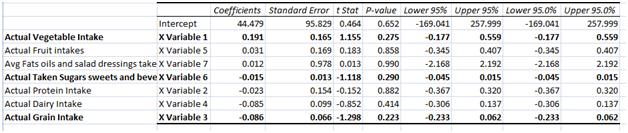
\includegraphics[scale=0.75]{excel-regression-food-groups} \\
\textbf{Regression on Actual Food Group Intake}\\
\hline
\end{tabular}

\begin{tabular}{|c|}
\hline
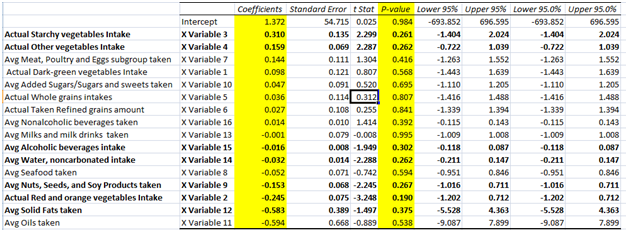
\includegraphics[scale=0.75]{excel-regression-food-subgroups}\\
\textbf{Regression on Actual Food Subgroup Intake} \\
\hline
\end{tabular}

\begin{tabular}{|c|}
\hline
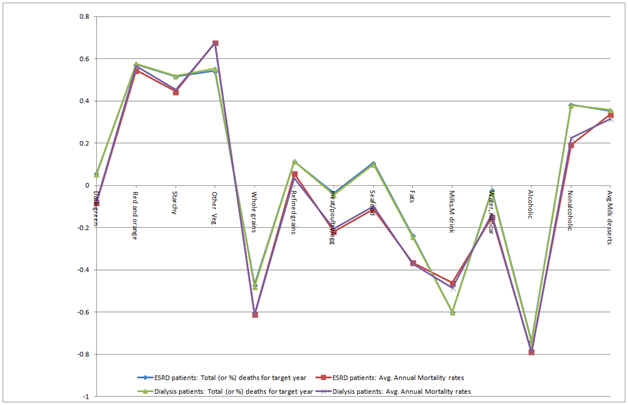
\includegraphics[scale=0.75]{line-plot-regression-exploratory.png}\\
\textbf{Line Plot for Regression outcome}\\
\hline
\end{tabular}

\begin{tabular}{|c|}
\hline
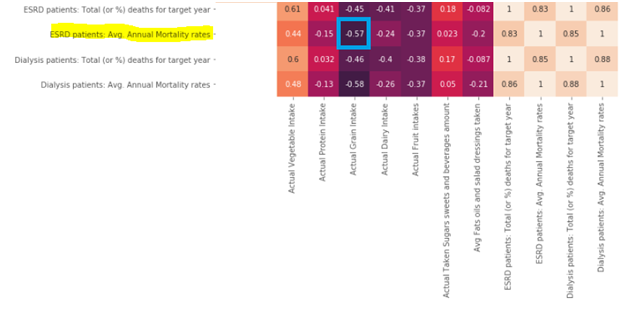
\includegraphics[scale=0.75]{heatmap-exploratory}\\
\textbf{Heatmap for exploration}\\
\hline
\end{tabular}
\caption{\textbf{Exploratory Analysis and Representative Output}}
\label{exploratory-output}
\end{figure}